% preamble
\documentclass{aastex631}

% imported packages
\usepackage{graphicx}
\usepackage{amsmath}
\usepackage{natbib}
\usepackage{longtable}

% some journal abbreviations for the bib file
\newcommand\AJ{AJ}%        % Astronomical Journal

% reset commands to set the line spacing
\renewcommand{\baselinestretch}{1.5}

\begin{document}

\title{Using Kuiper Observations to Explore the Temporal Evolution of the Tidal Disruption Event AT2024wsd}

\author[0000-0003-4537-3575]{noah franz}
\affiliation{Department of Astronomy \& Steward Observatory, University of Arizona}

\begin{abstract}
  Tidal disruption events (TDEs) occur when a star is torn apart by the tidal forces of a supermassive black hole. This event produces emission across the electromagnetic spectrum that varies on the timescales of months to years, depending on the wavelength of the emission. The origin of much of this emission is unknown. With the recent advent of all sky optical surveys, most TDEs have been discovered and followed up in the optical wavelengths, providing detailed light curves with temporal sampling on the order of days. However, to distinguish between potential optical emission models, it is essential to obtain a well sampled peak of the emission light curve. As a result, in this work we observe the TDE AT2024wsd with the Kuiper 61'' telescope located on Mt. Graham near optical peak, the first work to use this telescope for TDE followup. We find that our data has a relatively high signal-to-noise ratio of $\sim4-10$, depending on the filter, with only a 50s exposure time. From this data, we are also able to poorly constrain the rise rate of the system to be $\sim -0.05$ mag/day. This proof of concept study demonstrates that the Kuiper 61'' telescope can be an essential asset for TDE photometric followup with the inclusion of better time sampled data. 
\end{abstract}

\section{Introduction}
One of the most energetic events in the universe occurs when an unfortunate star approaches within the tidal radius of a supermassive black hole (SMBH). This is called a tidal disruption event (TDE) and was first theorized by \citet{hills1975}. \citet{rees1988} later predicted that the star would be tidally disrupted with $\sim$half of the material circularizing into an accretion disk around the SMBH and the other $\sim$half being ejected from the system as unbound debris. The material in the accretion disk should then produce bright, transient X-ray emission as it is accreted onto the SMBH. 

About a decade later, the first TDE candidates were discovered observationally as bright X-ray transients \citep{donley2002}. More recently, with the advent of large optical all sky surveys, TDEs were also discovered to emit at optical wavelengths \citep{iPTF,ZTF,panstarrstde}. The origin of this optical emission from TDEs remains an open question (2020 Decadel Survey, Subsection B-Q2a). The leading model is inverse compton scattering, typically called ``reprocessing'', of the high energy X-rays by gas in a torus surrounding the SMBH. Another possible model is that we are observing optical emission from the ejected material after it escapes the system and cools. \citet{gezari2021} provides a more detailed summary of these and additional models. 

This boom in the discovery of optically bright TDEs in the past $\sim$decade has resulted in $\sim200$ known TDEs to date, with a current discovery rate of $\sim10/yr$. The properties of the TDE emission provides a unique insight into the sub-parsec circumnuclei environment of galaxies and insights into the details of SMBH accretion \citep{holoien2020,Newsome2024}. In the optical, many of these properties are extracted using a combination of light-curve and spectral energy distribution fitting \citep{Mockler2019}. Even more, recent population analyses of the light-curves and spectral evolution of these TDEs show potential correlations between the optical TDE emission and physical properties of the system (e.g. \citet{vanVelzen2021}). However, more data is needed to verify these potential correlations and distinguish between the potential optical emission models.

Since these correlations are based on $\lesssim 100$ TDEs, they require further exploration with larger datasets to verify. As a result, following up TDEs both photometrically and spectroscopically is essential to further our understanding of the relation between TDE emission and the host galaxy and SMBH properties. The commonly used modeling softwares, like \citet{Mockler2019}, rely heavily on a well constrained peak in the light-curve of the TDE. This means that observing TDEs with numerous telescopes near peak brightness is essential for future analyses. Current all sky surveys, like the Zwicky Transient Facility \citep[ZTF]{ZTF}, provide well time sampled photometry with a few day cadence. But, other telescopes can help by observing the TDEs near peak and obtaining even better temporal sampling.

In this work, we observe the TDE AT2024wsd using the Kuiper 61'' telescope on Mt. Graham at, or near, peak brightness on the night of 2024-10-18 (local Arizona time); This is the first time the Kuiper 61'' has been used for such observations. AT2024wsd, (RA, Dec) = (05:26:38.320, -17:54:54.68), was originally discovered by ZTF on 2024-09-25 11:27:40 (UTC) with a magnitude of 20.0047 \citep{at2024wsd_discovery}. ZTF later classified AT2024wsd as a TDE based on the strong Hydrogen emission lines and blue nature of the spectrum \citep{at2024wsd_classification}. Our observations of AT2024wsd will contribute to improving the modeling of the TDE emission and will help extract improved constraints on properties of the system like the rise and decay times of the TDE emission, the SMBH mass, the tidally disrupted star mass, and accretion efficiency. In turn, these improved constraints will help us better understand the true origin of the optical emission from TDEs.

In \S\ref{sec:method}, we review our observing strategy and data reduction and calibration method. In \S\ref{sec:res}, we present the results and lessons learned from this unique opportunity. In \S\ref{sec:conclusion}, we summarize our method and results. All codes are available publicly at \url{https://github.com/noahfranz13/SO-Classes/tree/main/ASTR518/project}.

\section{Methods}\label{sec:method}
\subsection{Kuiper 61'' Observations}

\begin{table}
  \centering
  \caption{Observations Summary}
  \label{tab:obs}
  \begin{tabular}{lllrr}
    \hline
    Image Type & Filter & Start Time (UTC) & Exposure Time (s) & Number of Exposures \\
    \hline
    Target & Harris-B & 08:53:55.552 & 50.00 & 3 \\
    Target & Harris-V & 09:08:13.975 & 50.00 & 3 \\
    Target & Harris-R & 09:03:23.041 & 50.00 & 3 \\
    Target & Bessell-U & 08:58:18.912 & 50.00 & 3 \\
    Flat & Harris-B & 07:53:26.592 & 5.00 & 15 \\
    Flat & Harris-R & 07:46:32.588 & 5.00 & 30 \\
    Flat & Harris-V & 07:57:11.190 & 5.00 & 15 \\
    Flat & Bessell-U & 08:09:02.293 & 30.00 & 15 \\
    Bias & --- & 07:13:58.343 & 0.00 & 31 \\
    Dark & --- & 07:08:36.314 & 30.00 & 5 \\
    Dark & --- & 09:26:19.184 & 5.00 & 5 \\
    Dark & --- & 09:19:58.097 & 50.00 & 5 \\
    \hline
  \end{tabular}
\end{table}

We observed the TDE AT2024wsd with the Kuiper 61'' telescope on Mt. Graham on the night of October 18-19, 2024 (Local Date). A summary of the Target and Calibration observations is given in Table \ref{tab:obs}. We observed the target with the Mont4k CCD in the Harris- R, B, V and Bessell- U filters. The flat images were taken with the dome flat capability of the Kuiper 61'' telescope. The bias and dark images were taken using standard methods. While this telescope is not typically used for transient followup observations, our observing time for class provided a unique opportunity to test it's capabilities. 

\subsection{Data Calibration}
We performed standard bias calibration by stacking the bias images using an average with sigma clipping. The sigma clipping uses a $\pm 5 \sigma$ threshold to smooth the images over extreme outliers (e.g. hot pixels, cosmic rays, etc.). In future calibration steps, we use the same stacking parameters as used for the bias images. From the bias images, we estimate the read noise by subtracting off a random bias image from the master bias image ten times to create ten bias difference images. Since the bias images include both read noise and persistent detector signal, this renormalizes the bias images and removes extraneous outliers, leaving behind just the extra current due to read noise. Finally, we take the standard deviation of all of these images to find the read noise and convert from ADU to electrons using the gain  $G=3.1~e/ADU$ of Mont4k\footnote{\url{https://james.as.arizona.edu/~psmith/61inch/CCD/basicinfo.html}}.

After stacking the bias images, we apply the master bias image to each dark image to remove the CCD bias and leave behind just the dark current. We then stack the dark images by exposure time, leaving us with a master 5s, 30s, and 50s dark image. This is necessary for calibrating the Flat images, which were taken at 5s and 30s, and target images, which were taken at 50s. From the dark images, we estimate the dark noise by computing the mean pixel count for each dark image and then performing a linear fit to the mean pixel count as a function of exposure time. This gives us a dark current in electrons per pixel per second. Since dark current is a poissonian process, we simply take the square root of the dark current to find the dark noise (i.e. the shot noise of the dark current) and convert from ADU to electrons using the gain $G=3.1~e/ADU$ of Mont4k. 

To calibrate the flat images, we apply the master bias and then the master dark corrections. For the Harris- B, R, V flat images we use the 5s dark correction and for the Bessell-U flat image we use the 30s dark correction. We then stack the flat images to create one flat for each filter. The flats are not used to estimate any of the noise sources.

\begin{figure}[!h]
  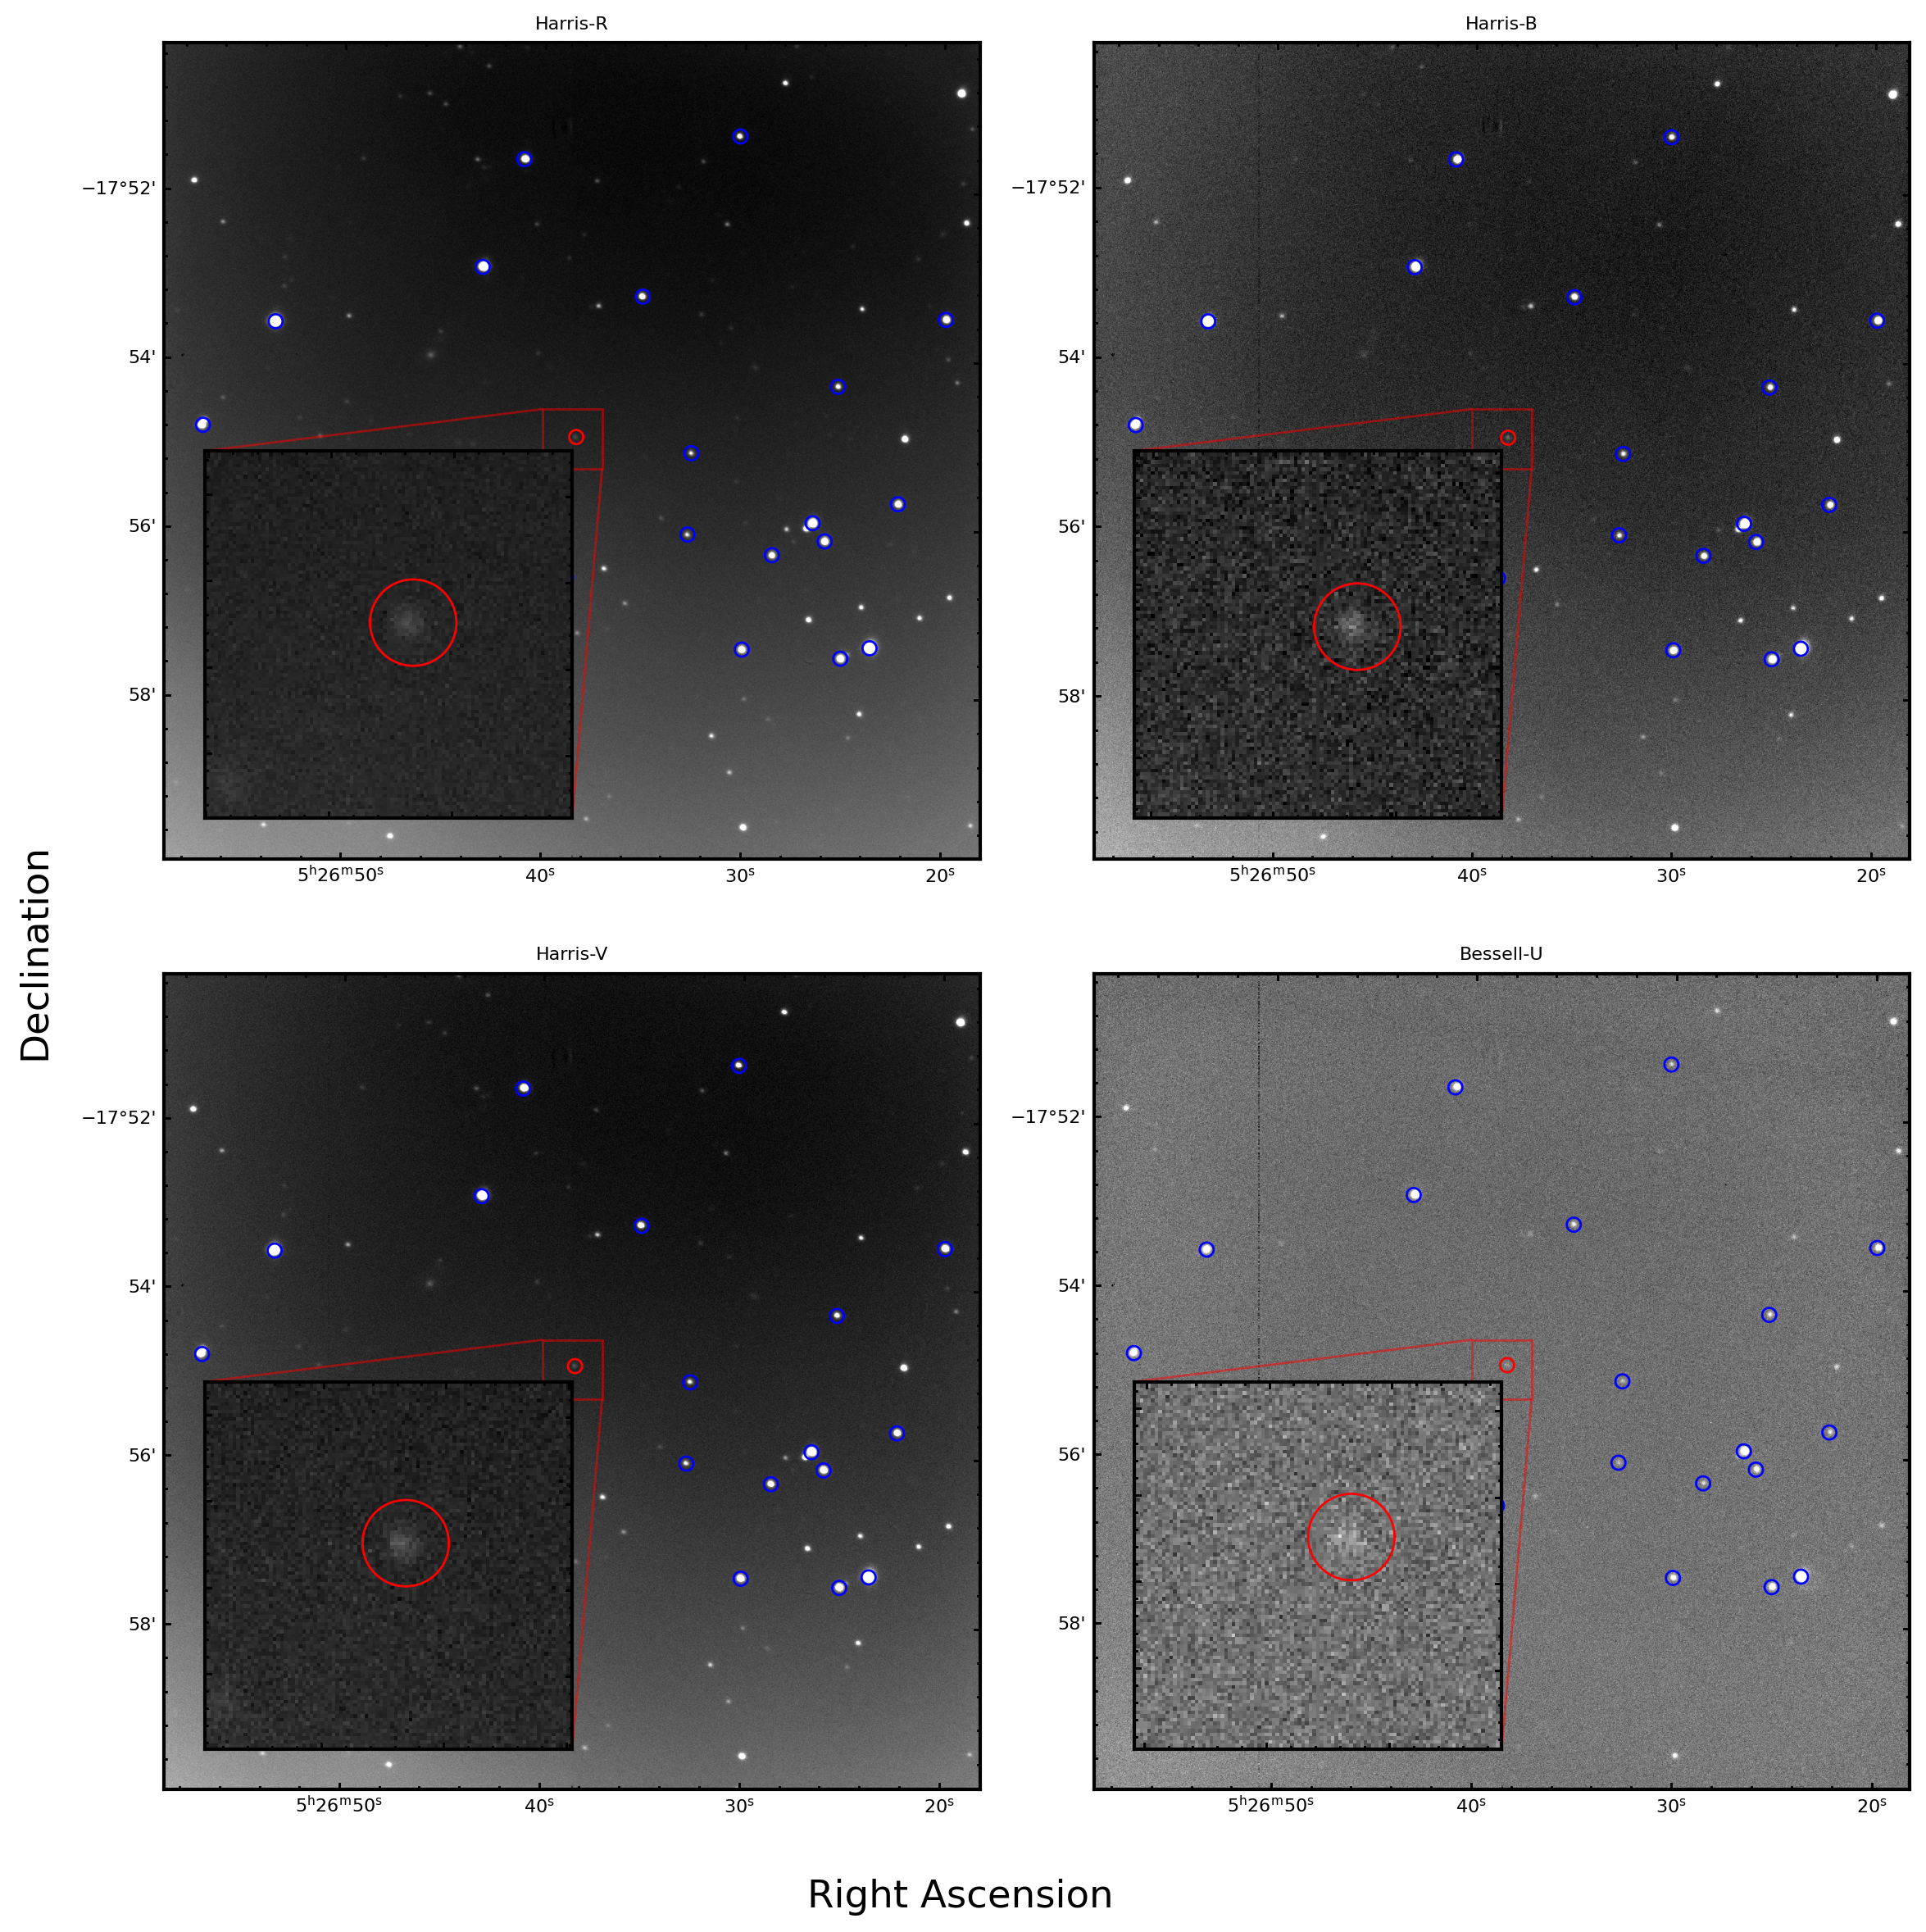
\includegraphics[width=\textwidth]{../analysis/fcal-images.png}
  \caption{Post-reduction stacked images in the four filters we observed in. In the background image, the red square surrounds the zoom in region which includes the aperture, the red circle, overlayed on top of our target. The blue circles are the apertures on the foreground sources used for the flux calibration.}
  \label{fig:targ}
\end{figure}

Finally, we apply all of these calibrations to the target images. First, we bias correct the target images using the master bias. Then, we subtract the 50s master dark image from the target images. We apply the flat correction to each bias and dark corrected target image for the corresponding filter. Then, we stack all of the corrected target images by filter to give 4 science images. We then use \texttt{astrometry.net} \citep{lang2010} to compute the WCS solutions for each image. From these reduced images, we remove the chip gap by using a scanning method with a tophat kernel that averages over the 4 pixels on either side of the gap. This leaves us with the images in Figure \ref{fig:targ}. 

\subsection{Signal Extraction and Flux Calibration}
We compute the sum of the ADU counts from the target using an circular aperture centered at the target coordinates, (RA, Dec) = (05:26:38.320, -17:54:54.68), with a 5'' radius. This includes all of the pixels nearby the target with counts that visibly rise above the background and noise. The apertures for each filter are shown as red circles in Figure \ref{fig:targ}. The counts from each aperture are shown in Figure \ref{fig:aperture-counts}. These count histograms appear very Gaussian which likely means we are pushing up against the point spread function (PSF) of the telescope and instrument. This means that, as expected, our target can be treated as a point source since it fills the PSF of the telescope. To find the sum of the ADU counts within the aperture, we simply integrate over these count histograms. 

\begin{figure}
  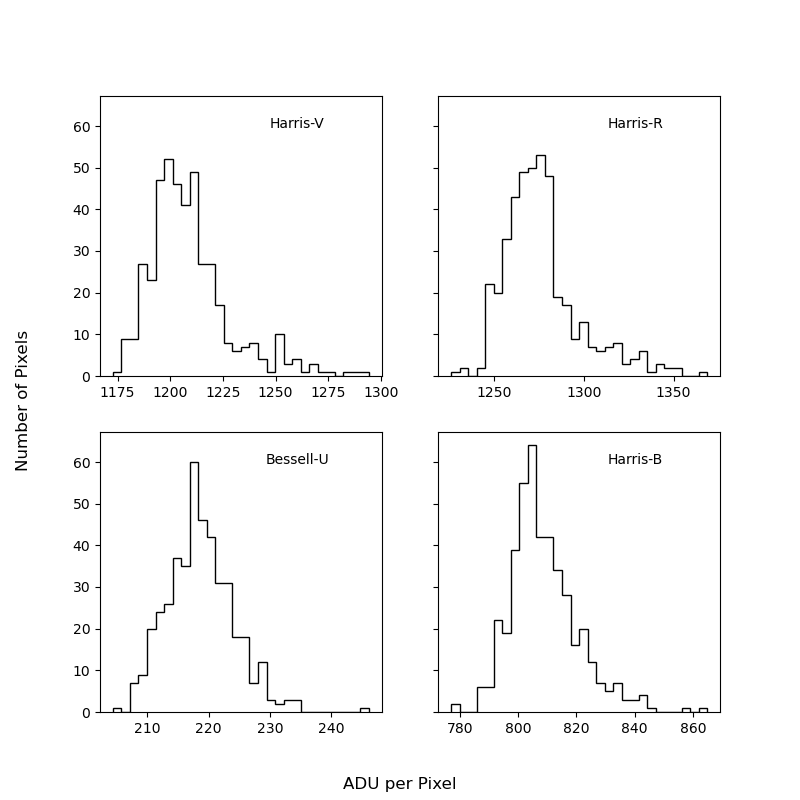
\includegraphics[width=\textwidth]{../analysis/aperture-counts-hist.png}
  \caption{Distributions of ADU counts in the target apertures for each filter. Each histogram is approximately Gaussian indicating that the target fills the point spread function of the telescope.}
  \label{fig:aperture-counts}
\end{figure}

We convert the sum of the counts from the target plus background to electrons using the gain $G=3.1~e/ADU$. Then, to convert from electrons to photons, we assume a throughput $T=85.78\%$ which is derived assuming the primary mirror has a $93\%$ reflectivity and that there are four other optics between the primary mirror and detector that each have an individual throughput of $98\%$. Combining these gives a throughput $T=(0.93)(0.98)^4=0.8578$. We also assume a constant quantum efficiency $Q=70\%$\footnote{\url{https://lavinia.as.arizona.edu/~tscopewiki/doku.php?id=public:catalinas:bigelow:kuiper_61:mont4k}} that is derived from the approximate average quantum efficiency from 300-700nm. Using the throughput and quantum efficiency, we convert from electrons to photons incident on the telescope by multiplying the electron counts by $1/(T \times Q)$. These counts, in ADU, electrons, and photons are given in Table \ref{tab:res}.

To estimate the background signal, we use an annulus aperture centered on the target coordinates with an inner radius of 5'' and outer radius of 10''. We chose to use an annulus to estimate the background because, by visual inspection of the images, the background rate varies by $\sim300$ counts ($\sim25\%$) across the image. This is likely because the target was near the setting moon which created a gradient of background illumination. Therefore, we want a local estimate of the background rather than a global one. After integrating over the counts in the annulus, we take the average to find the background counts per pixel. We then subtract the background counts, multiplied by the area of the target aperture, from the target aperture counts to find the signal coming just from the target itself. We follow the same procedure as with the target aperture to convert from ADU to electrons and photons. The background estimation and subtraction results are in Table \ref{tab:res}.

Once we have a background subtracted signal, we need to convert from photon counts to physical units. To do this, we query the VizieR data service for Johnson/Cousins magnitudes in our field of view. We follow the same procedure as used for the target for each of these stars in the field of view: 1) place a 5'' aperture  over each source and find the sum of the counts; 2) Find and subtract the background using an annulus with a 5'' inner radius and 10'' outer radius; and 3) Convert from ADU to electrons and photons. The aperture placed on each of these foreground stars is shown as a blue circle in Figure \ref{fig:targ}. We did this for 19 foreground stars and the results of the aperture photometry and background annulus estimation for one source are given in Table \ref{tab:res}.

Each of these foreground stars has synthetic Johnson/Cousins magnitudes generated from the Gaia BP and RP mean spectra of the sources \citep{gaiadr3,gaiadr3_syntphot} (VizieR catalog I/360/syntphot). Note that we choose to use the Johnson/Cousins filter system since it is very similar to the Harris and Bessell filters but a more common standard. This, of course, introduces a level of systematic uncertainty into our magnitude calculation but this is negligible compared to the  uncertainties on our flux calculations. From these synthetic magnitudes, we find the zero point, $f_0$ of each filter using equation \ref{eq:f0},

\begin{align}
  f_{0,\gamma} = f_\gamma \times 10^{0.4 * m_\lambda},\label{eq:f0}
\end{align}

\noindent where $f_\gamma$ is the photon count flux and $m_\lambda$ is the synthetic magnitude of the source in a given filter.

\noindent We take the median of the computed zero points from each of these foreground stars to find a single zero point for the Mont4k detector. We choose to use the median to make our zero point calculation robust to outliers like variable stars or possible contaminating galaxies. The calculated zero points in photon counts are listed in Table \ref{tab:res}. Using the computed zero points we calculate the magnitude for each filter of our source using the standard flux-magnitude equation,

\begin{align}
  m_\lambda = -2.5\log_{10}\left(\frac{f_\gamma}{f_{\gamma,0}}\right).
\end{align}

\noindent We compute the uncertainty in these magnitudes using standard error propagation on the noise in the photon count flux,

\begin{align}
  \sigma_m \approx \frac{\ln(10)}{2.5} \frac{\sigma_{f_\gamma}}{f_\gamma} .
\end{align}

\noindent The computed apparent magnitudes with uncertainty are given in Table \ref{tab:res} and shown in Figure \ref{fig:lc} with respect to other public photometry of this tidal disruption event.

\subsection{Light-Curve Modeling}
To compare the magnitudes measured at Kuiper to other public photometry we pull all of the available photometry on the Transient Name Server page for AT2024wsd\footnote{https://www.wis-tns.org/object/2024wsd} which consists mostly of Zwicky Transient Facility (ZTF) preliminary detections. The Kuiper photometry and public photometry are shown for comparison in Figure \ref{fig:lc}. We also query the Asteroid Terrestrial-impact Last Alert System (ATLAS) forced photometry service for archival photometry of this target. The ATLAS query revealed all nondetections, which are also shown in Figure \ref{fig:lc}. To compare the public photometry to our Kuiper data, we assume that the measurements in the Johnson/Cousins filters are similar to those made in the ZTF b, g, and r filters because the effective wavelengths tend to be within a few hundred angstroms. There are obviously limitations to this assumption but it is our only option given the lack of {\it public} photometry for this object. There is no public photometry available for the Bessell-U filter so we are unable to derive rise rates for this filter.

Since there are only one or two additional public photometry points for AT2024wsd, we are only able to apply a simple linear fit to the brightening of the transient. We do this by using a $\chi^2$ fit of a linear model $m = m_0 + kt$, where $k$ is the brightening rate in magnitudes per day, to the data. This fit gives us a brightening rate of the transient and, assuming that we observed at or near peak brightness, a rise time for the brightening of the transient. 

\section{Results \& Discussion}\label{sec:res}
\subsection{Observational Results}

\begin{table}
  \centering
  \caption{Reduction Results}
  \label{tab:res}
  \begin{longtable}{lllll}
    \hline
    Filter & Harris-R & Harris-B & Harris-V & Bessell-U \\
    \hline
    Source Aperture Sum (ADU) & 554351.81 & 351531.39 & 524268.83 & 94429.37 \\
    Source Aperture Sum (e) & 1718490.61 & 1089747.30 & 1625233.38 & 292731.06 \\
    Source Aperture Sum ($\gamma$) & 2861956.85 & 1814854.11 & 2706647.21 & 487511.34 \\
    \hline
    Background Annulus Sum (ADU) & 548693.02 & 348232.62 & 521197.05 & 93495.58 \\
    Background Annulus Sum (e) & 1700948.36 & 1079521.11 & 1615710.86 & 289836.31 \\
    Background Annulus Sum ($\gamma$) & 2832742.16 & 1797823.52 & 2690788.50 & 482690.45 \\
    \hline
    Dark Noise ($\sigma_D$; ADU/pixel) & 0.29 & 0.29 & 0.29 & 0.29 \\
    Dark Noise ($\sigma_D$; e/pixel) & 0.51 & 0.51 & 0.51 & 0.51 \\
    \hline
    Read Noise ($\sigma_R$; ADU/pixel) & 3.15 & 3.15 & 3.15 & 3.15 \\
    Read Noise ($\sigma_R$; e/pixel) & 9.76 & 9.76 & 9.76 & 9.76 \\
    \hline
    Target Signal ($f_e$; e) & 17542.25 & 10226.19 & 9522.52 & 2894.75 \\
    Target Signal ($f_\gamma$; $\gamma$) & 29214.69 & 17030.59 & 15858.71 & 4820.89 \\
    Noise on Target (e) & 1326.70 & 1063.67 & 1291.08 & 578.25 \\
    SNR for Target & 13.22 & 9.61 & 7.38 & 5.01 \\
    \hline
    Sample Flux Cal. Aperture Sum (ADU)\footnote{This from 1 of the 19 foreground stars used to estimate the zero point. The others are available upon request.} & 786324.66 & 413693.58 & 692494.86 & 102921.67 \\
    Sample Flux Cal. Background Annulus Sum (ADU) & 583842.18 & 356051.85 & 543212.76 & 94262.53 \\
    Sample Flux Cal. Signal (ADU) & 202482.48 & 57641.73 & 149282.10 & 8659.14 \\
    Sample Flux Cal. Signal (e) & 627695.68 & 178689.35 & 462774.51 & 26843.33 \\
    Sample Flux Cal. Signal ($\gamma$) & 1045358.02 & 297587.43 & 770699.97 & 44704.61 \\
    Sample Flux Cal. Noise (e) & 1574.56 & 1150.69 & 1479.32 & 600.58 \\
    \hline
    Zero Point ($10^{12}f_0$; $\gamma$) & 0.44 & 0.32 & 0.47 & 0.05 \\
    Apparent Magnitude & 17.95 & 18.18 & 18.67 & 17.51 \\
    Apparent Magnitude Error & 0.07 & 0.10 & 0.12 & 0.18 \\
    \hline
  \end{longtable}
  \centering
  \vspace{-0.75cm}
\end{table}
A summary of our data reduction and zero point calibration results is in table \ref{tab:res}. From these calibrations, we compute a signal-to-noise ratio, derived both theoretically (\S\ref{sec:snr_theory}) and observationally (\S\ref{sec:snr_obs}), in the subsequent sections.  

\subsubsection{Theoretical SNR Calculations}\label{sec:snr_theory}
Prior to observing, we computed the theoretical observing time using the standard SNR equation, equation \ref{eq:snr},

\begin{align}
  SNR = \frac{N_e}{\sqrt{N_e + n_{pix}f_{bkgd}t_{exp} + n_{pix}t_{exp}D + n_{pix}R^2 }}, \label{eq:snr}
\end{align}
where $f_e$ is the electron count flux, $n_{pix}$ is the number of pixels in the aperture, $f_{bkgd}$ is the background electron count flux, $t_{exp}$ is the exposure time, $D$ is the dark current, and $R$ is the read noise. To find the exposure time, we use the sky brightness estimate, $m_{bkgd}=22 mag/as^2$; standard read noise, $R=5~e$; dark current, $D=16.6 e/pix/hr$; gain $G=3.1 e/ADU$; quantum efficiency, $Q=0.88$; and throughput, $T=0.8578$. Using these values, we solve equation \ref{eq:snr} as a quadratic and find that for an SNR of 10 for a target with visible magnitude $V\sim18$, the exposure time on the Kuiper telescope with the Mont4k detector is $t_{exp} \sim 0.01s$. 

\subsubsection{Observed SNR Calculation}\label{sec:snr_obs}
To observationally estimate the SNR of our measurement of AT2024wsd, we use a modified version of equation \ref{eq:snr},

\begin{align}
  SNR = \frac{N_e}{\sqrt{N_e+N_{bkgd}+n_{pix}\left(D + R^2\right)}},
\end{align}

\noindent where we combine the background noise term into simply the counts in the background annulus, $N_{bkgd}$. Filling in values from Table \ref{tab:res}, we find the SNRs per filter given in the last row of Table \ref{tab:res}. These SNRs are comparable to the SNR$\sim10$ used in the theoretical calculations. However, we used three 50s exposures in each filter instead of the theoretical exposure time $t\sim0.01s$. This is likely because our noise is significantly dominated by our background and shot noise rather than the read and dark noise. In particular, the poissonian background noise is significantly higher than we theoretically estimated, likely because the target was very close to the moon. Additionally, but likely less of a cause of this discrepancy, is that both the dark and read noise seem to be $\sim2$ times larger than the values presented in the Mont4k documentation. This is most likely because those values were found in an isolated environment rather than true observing environment.  

\subsection{Zero Point Calibration and Light-Curve Fit Results}
\begin{figure}
  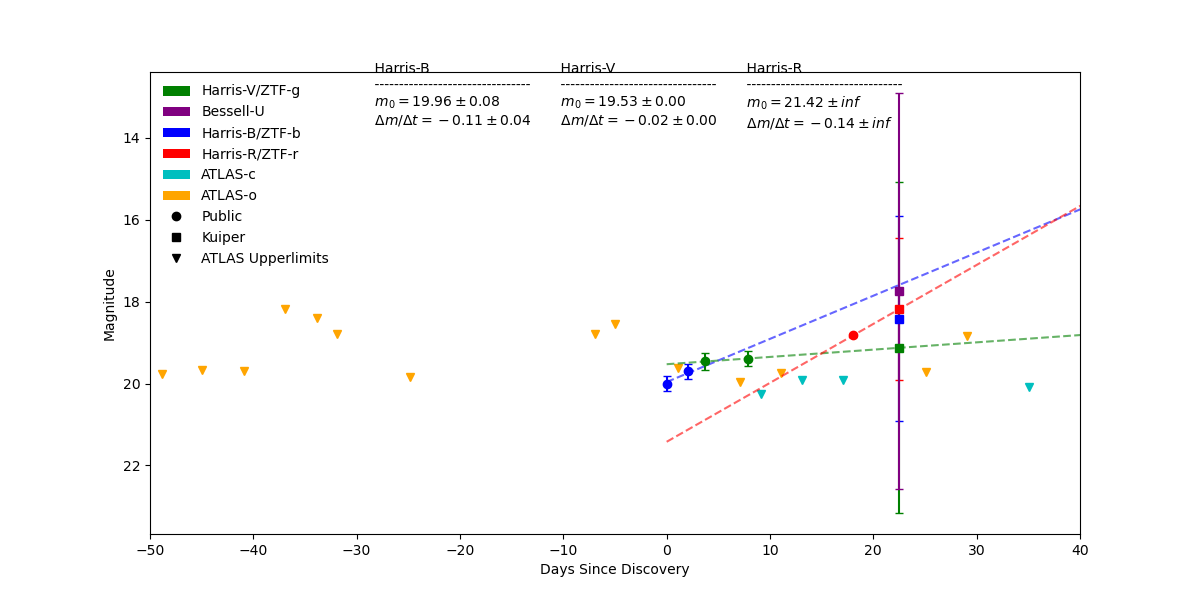
\includegraphics[width=\textwidth]{../analysis/lightcurve.png}
  \label{fig:lc}
  \caption{Light curve, or magnitude as a function of days since discovery, of both the publicly available photometry (circles) and photometry (squares) from this work. ATLAS upperlimits are shown as downward facing triangles in both their cyan filter and orange filter. The best fit linear rise models are shown as dashed lines where the color corresponds to the color of the data points it is a fit for.}
\end{figure}

The magnitudes and photon count flux zero points that we computed are given in Table \ref{tab:res}. These results are also shown in comparison to publicly available photometry in Figure \ref{fig:lc}. As expected, the magnitudes we computed are brighter than the publicly released magnitudes because the transient brightness was likely near peak brightness during our observation.

The best linear model to the data is displayed in Figure \ref{fig:lc} as dashed lines. The results of the fits, with uncertainties, are given as text in the top of the figure. All fits are relatively poorly constrained given the lack of data. But, in particular, the red filter data are very poorly constrained with only two photometry points. Therefore, we place limited faith in the rise rates presented in Figure \ref{fig:lc}. Even still, using these fits, we can estimate the rise time of this TDE as $t_{rise} \sim 20$ days, an especially interesting quantity since past works have shown that it can be related to the supermassive black hole mass \citep{vanVelzen2021}. However, this rise time should be considered a lower limit on the true rise time since our data does not include any photometry on the decay of the light curve.

\subsection{Limitations and Lessons Learned}

The primary lesson learned from this work is that the exposure time computed with the theoretical SNR equation \ref{eq:snr} is likely unreliable for the Kuiper 61'' telescope based on the standard noise sources. In the future, it would be beneficial to include a better estimate of the background brightness and slightly higher values for the read and dark noise.

Another important limitation of this work is the comparison of the Harris and Bessell filter system to the Johnson/Cousins and ZTF filter systems. Ideally, we would need to perform a bolometric correction to apply to the Harris and Bessell filters on Mont4k to convert them properly to the Johnson/Cousins and ZTF filters. This is especially necessary because the Harris and Bessell filters are non-standard, unlike the Johnson/Cousins filter system. Future work would include a more robust analysis of this conversion, including the bolometric conversion, rather than assuming the Harris and Bessell filters are similar to the Johnson/Cousins system. 

Another important lesson from this is that the Kuiper telescope is not optimized for photometric follow up of transient events. This is because we would need nearly nightly, or at least weekly, time on the telescope to improve our temporal sampling of the light-curve. Or, using some Kuiper observations in combination with the more complete, but private, ATLAS and ZTF datasets. In the end, because ZTF and ATLAS follow up these transients on a nightly basis, it would probably make more sense to let them get the photometry and we use Kuiper for spectrographic followup and classification of transients in the future.   

Finally, It is important to note that in the literature the rise rate and rise time of tidal disruption events is typically found with a gaussian fit to the data \citep{gezari2021, vanVelzen2021}. However, with our limited dataset, such a fit would be nearly impossible to perform. In the future, it would, once again, be beneficial to include a better temporally sampled dataset to better constrain the peak, and therefore rise time, of the light-curve. 

\section{Conclusions}\label{sec:conclusion}

In this work we used the Kuiper 61'' telescope to perform photometric follow up of a tidal disruption event, AT2024wsd, for the first time. We observed the TDE in four filters, Harris- B, V, R and Bessell-U, with 3 exposures, each with an exposure time of 50s. We then reduced the images using standard procedures. We calibrated the flux of AT2024wsd by deriving a photon count zero point using publicly available Johnson/Cousins magnitudes of foreground stars.

The results of these observations are explained in detail in \S\ref{sec:res} and given in Table \ref{tab:res}. Our signal to noise ratio ranges from $\sim4$ to $\sim10$ depending on the filter used. The magnitudes we found are about 1 mag brighter than previous public photometry. This was expected since the rise time of TDE optical emission tends to be around a month and we were observing AT2024wsd about 3 weeks after initial discovery. Using a combination of our photometry and previous public photometry, we find a gradual rise to the approximate peak brightness around $20$ days after discovery of about $-0.05$ mag/day, depending on the filter used. This rise rate was derived using a linear fit to our limited dataset and is poorly constrained. This rise time reported here should be treated as a lower limit since we have no photometry during the light-curve decay.

Overall, this work has shown that the Kuiper 61'' telescope can be a valuable asset for photometric follow up of tidal disruption events. After the Kuiper telesope is equipped with a spectrograph, future work should also explore the use of the telescope for specotroscopic follow up. Future analyses should also work with the ZTF and ATLAS collaborations to generate a better temporally sampled light curve of the transient event. Or, similarly, convert the Kuiper telescope to a robotic observatory to scan the entire sky each night (or every few nights). This will allow for more detailed modeling and the extraction of more interesting parameters of the disrupting system, like the SMBH mass and accretion properties. 

\software{
  \citet{lang2010},
  \citet{photutils},
  \citet{ccdproc},
  \citet{astropy:2022},
  \citet{numpy},
  \citet{pandas-ds},
  \citet{pandas-zenodo}
}

\bibliographystyle{aasjournal}
\bibliography{main}

\end{document}

%%% Local Variables:
%%% mode: LaTeX
%%% TeX-master: t
%%% End:
